\documentclass{article}
\usepackage[slovak]{babel}
\usepackage{graphicx}
\begin{document}
\title {\textbf{Laboratórny protokol - Rýchlosť rastu fazule a žeruchy}}
\author{Adam Jenča}
\setlength{\tabcolsep}{18pt}
\renewcommand{\arraystretch}{1.5}
\maketitle
\section{Úvod}
V tomto experimente sme mali za úlohu zistiť priemernú rýchlosť rastu fazule a žeruchy.
Priemerná rýchlosť $v_p$ je definovaná ako $\frac{s_t}{t_t}$, kde $s_t$ predstavuje celkovú dráhu a $t_t$ celkový čas.
\section{Pomôcky a postup}
\subsection{Pomôcky}
\begin{itemize}
\item{Semená žeruchy a fazule}
\item{Pôda}
\item{Voda}
\item{Nádoby (2x)}
\item{Meradlo}
\item{Špajdľa na uchytenie fazule}
\end{itemize}
\subsection{Postup}
\begin{enumerate}
	\item Pripravíme si nádoby a spravíme do ich dna dierky na odtečenie vody.
	\item Nádoby naplníme ich do $\frac{2}{3}$ pôdou.
        \item Do jednej nádoby dáme 10-15 semien žeruchy, do druhej dáme 3-5 semien fazule.
	\item Nádoby označíme podľa toho, čo je v nich zasiate.
	\item Nádoby doplníme pôdou približne do $\frac{5}{6}$ objemu. Pôdu jemne utlačíme.
        \item Do nádoby s fazuľou zapichneme špajdľu.
        \item Obe rastliny polejeme vodou.
        \item Rastliny necháme na teplom, slnečnom mieste, pravidelne polievame a meriame ich výšku.
\end{enumerate}
\section{Tabuľky a výpočty}
\begin{center}
\begin{tabular}{|c|c|c|c|c|}
	\hline
	$t[d]$ & $s_{z}[mm]$ & $s_{f}[mm]$ & $\Delta_{s_z}[mm]$ & $\Delta_{s_f}[mm]$\\
	\hline
	$0$&$0$&$0$&$0$&$0$\\
	\hline
	$1$&$5$&$0$&$5$&$0$\\
	\hline
	$3$&$12$&$0$&$7$&$0$\\
	\hline
	$4$&$15$&$0$&$3$&$0$\\
	\hline
	$7$&$23$&$0$&$8$&$0$\\
	\hline
	$9$&$27$&$0$&$4$&$0$\\
	\hline
	$11$&$29$&$0$&$2$&$0$\\
	\hline
	\multicolumn{5}{|c|}{Tu sa rast  žeruchy zastavil.}\\
	\hline
	$14$&$29$&$0$&$0$&$0$\\
	\hline
	$16$&$29$&$0$&$0$&$0$\\
	\hline
	\multicolumn{5}{|p{12.5cm}|}{Vysvetlivky: $t[d]$ - Čas v dňoch, $s_{z}[mm]$ - Výška žeruchy v mm, $s_{f}[mm]$ - Výška fazule v mm, $\Delta_{s_z}[mm]$ - Rozdiel vo výške žeruchy oproti predch. meraniu, $\Delta_{s_f}[mm]$ - Rozdiel vo výške fazule oproti predch.meraniu}\\
	\hline
\end{tabular}
\end{center}
Ako vidno, fazuľa vôbec nevyrástla.
Žerucha vyrástla o 29 mm za 16 dní, takže rástla $v_p$ 1.8125 $\frac{mm}{d}$
\newpage
\section{Grafy}
\subsection{Graf dráhy}
	\begin{figure}[h!]
		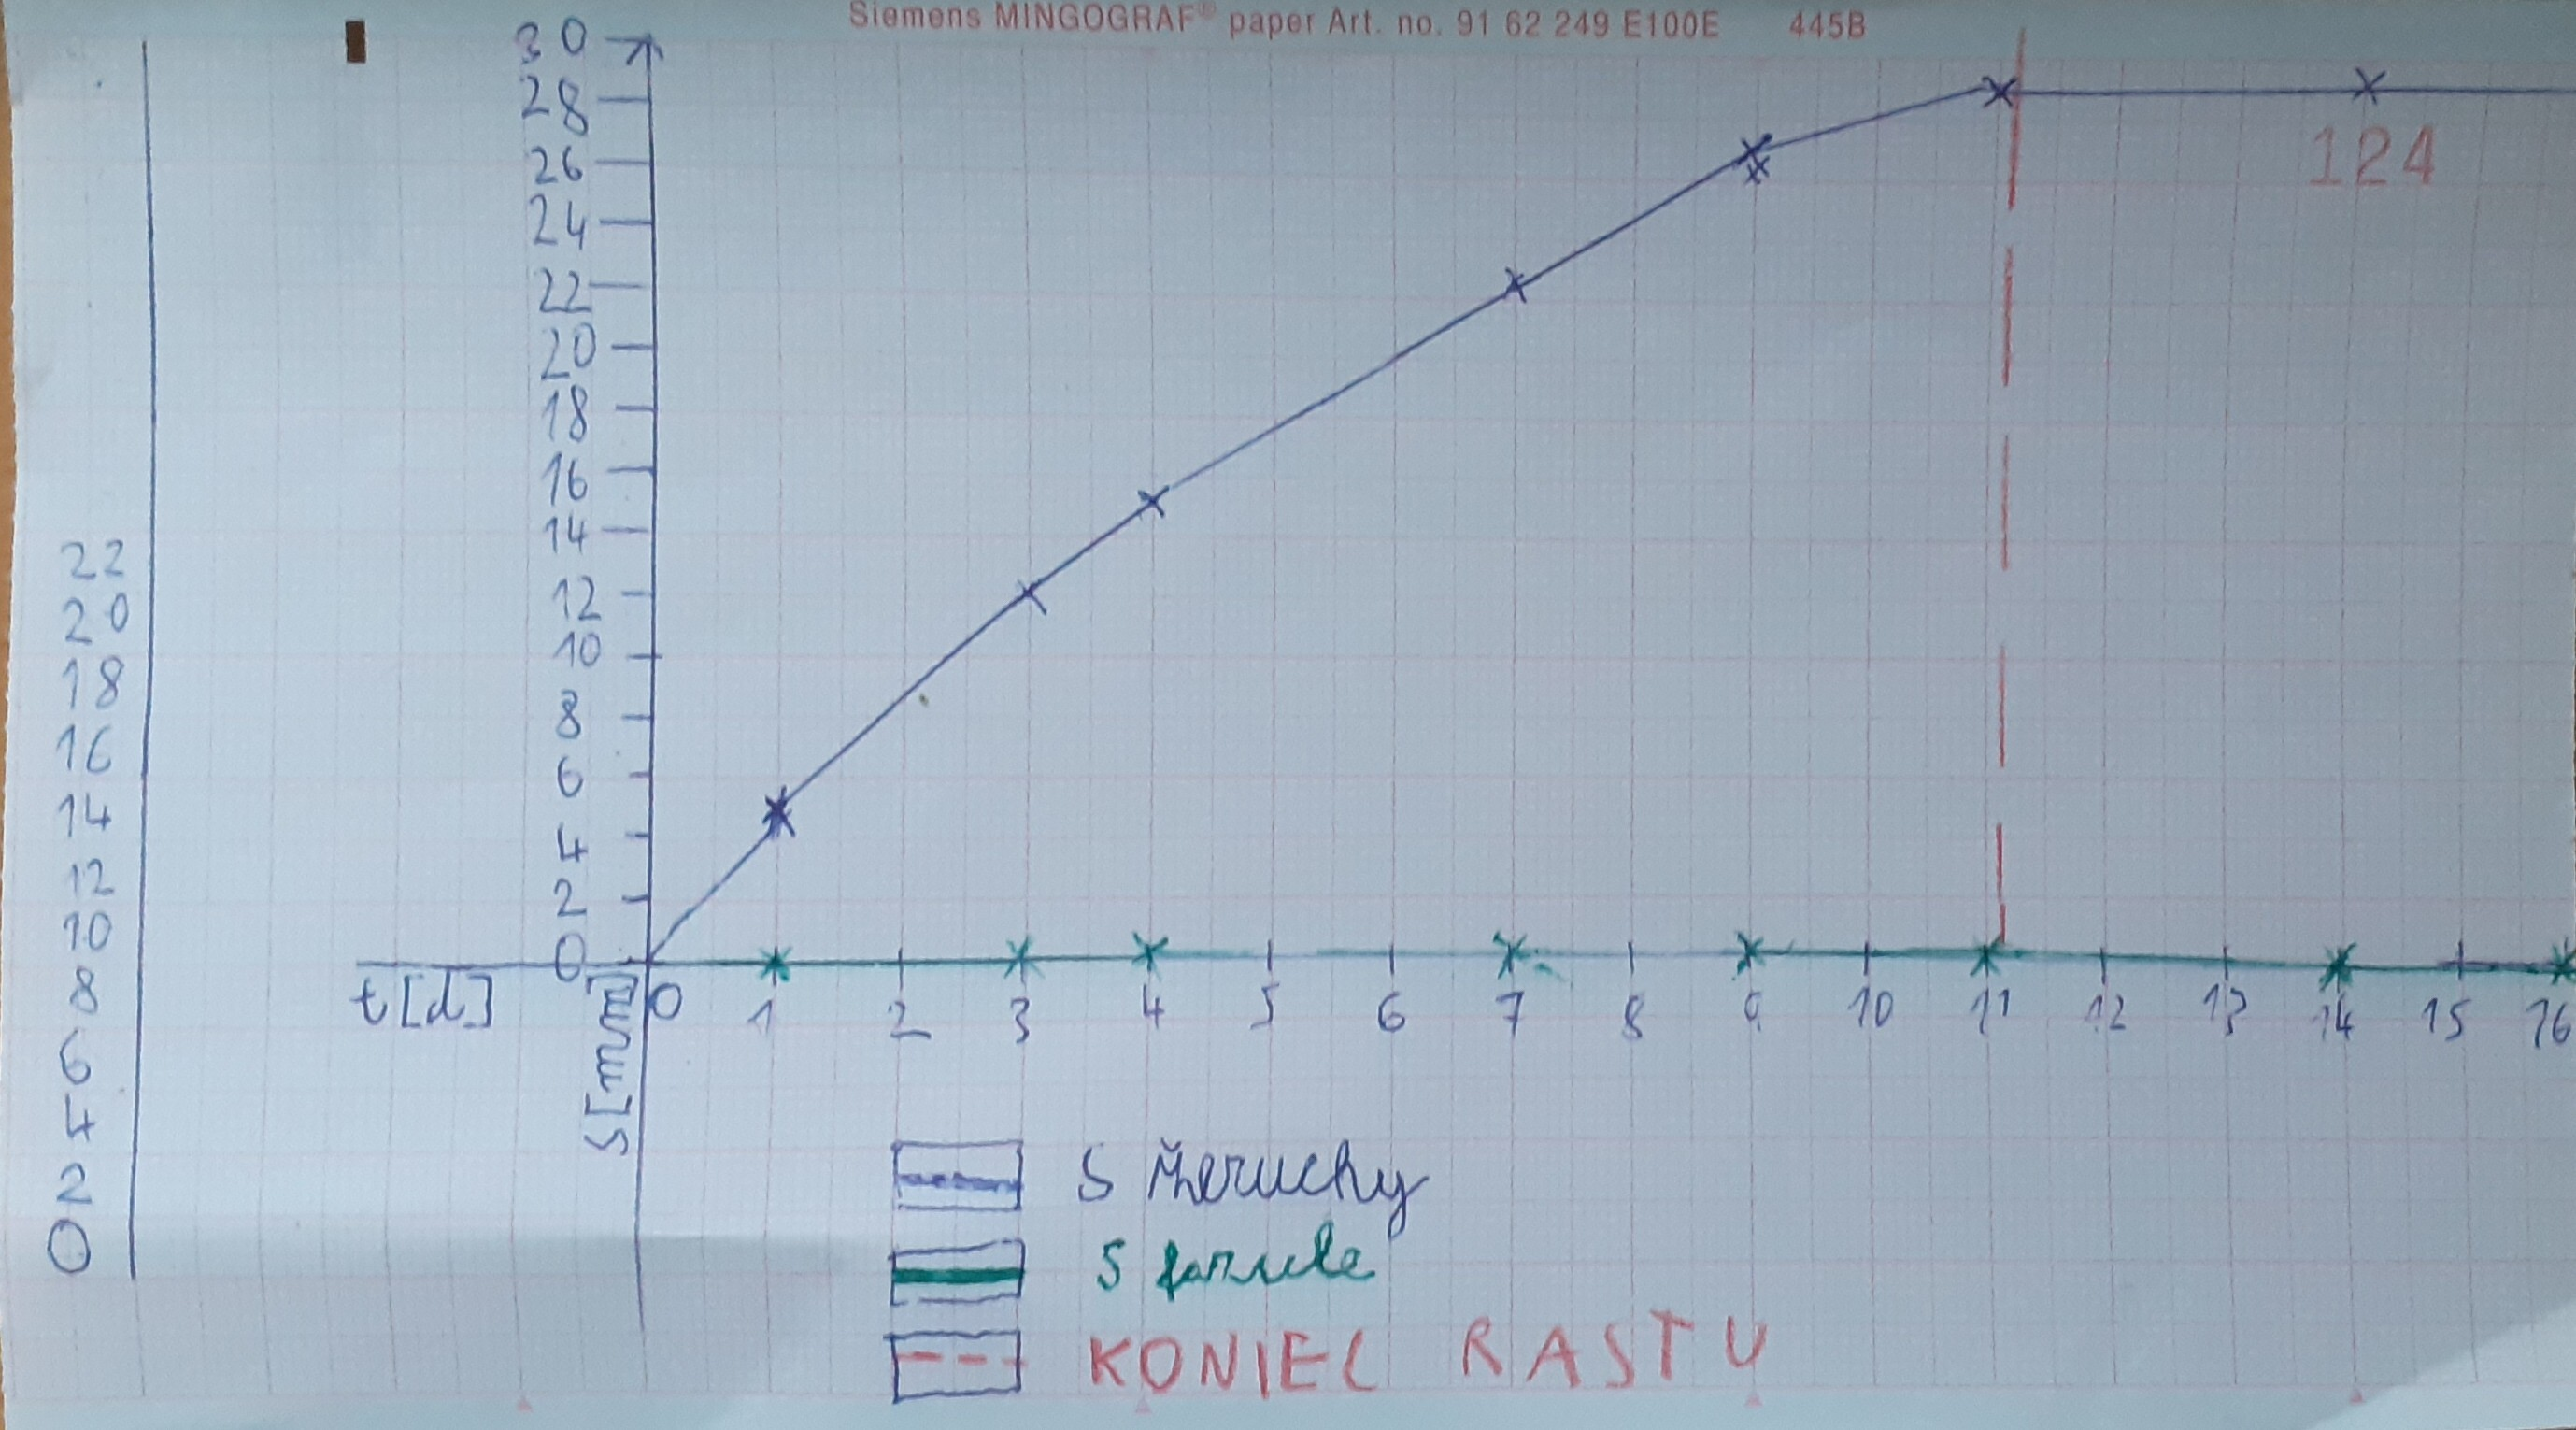
\includegraphics[width=10cm]{graf-1.jpeg}
	\caption{Graf $s_z$ a $s_f$ v závislosti od $t$}
\end{figure}
\subsection{Graf rýchlosti}
\begin{figure}[h!]
		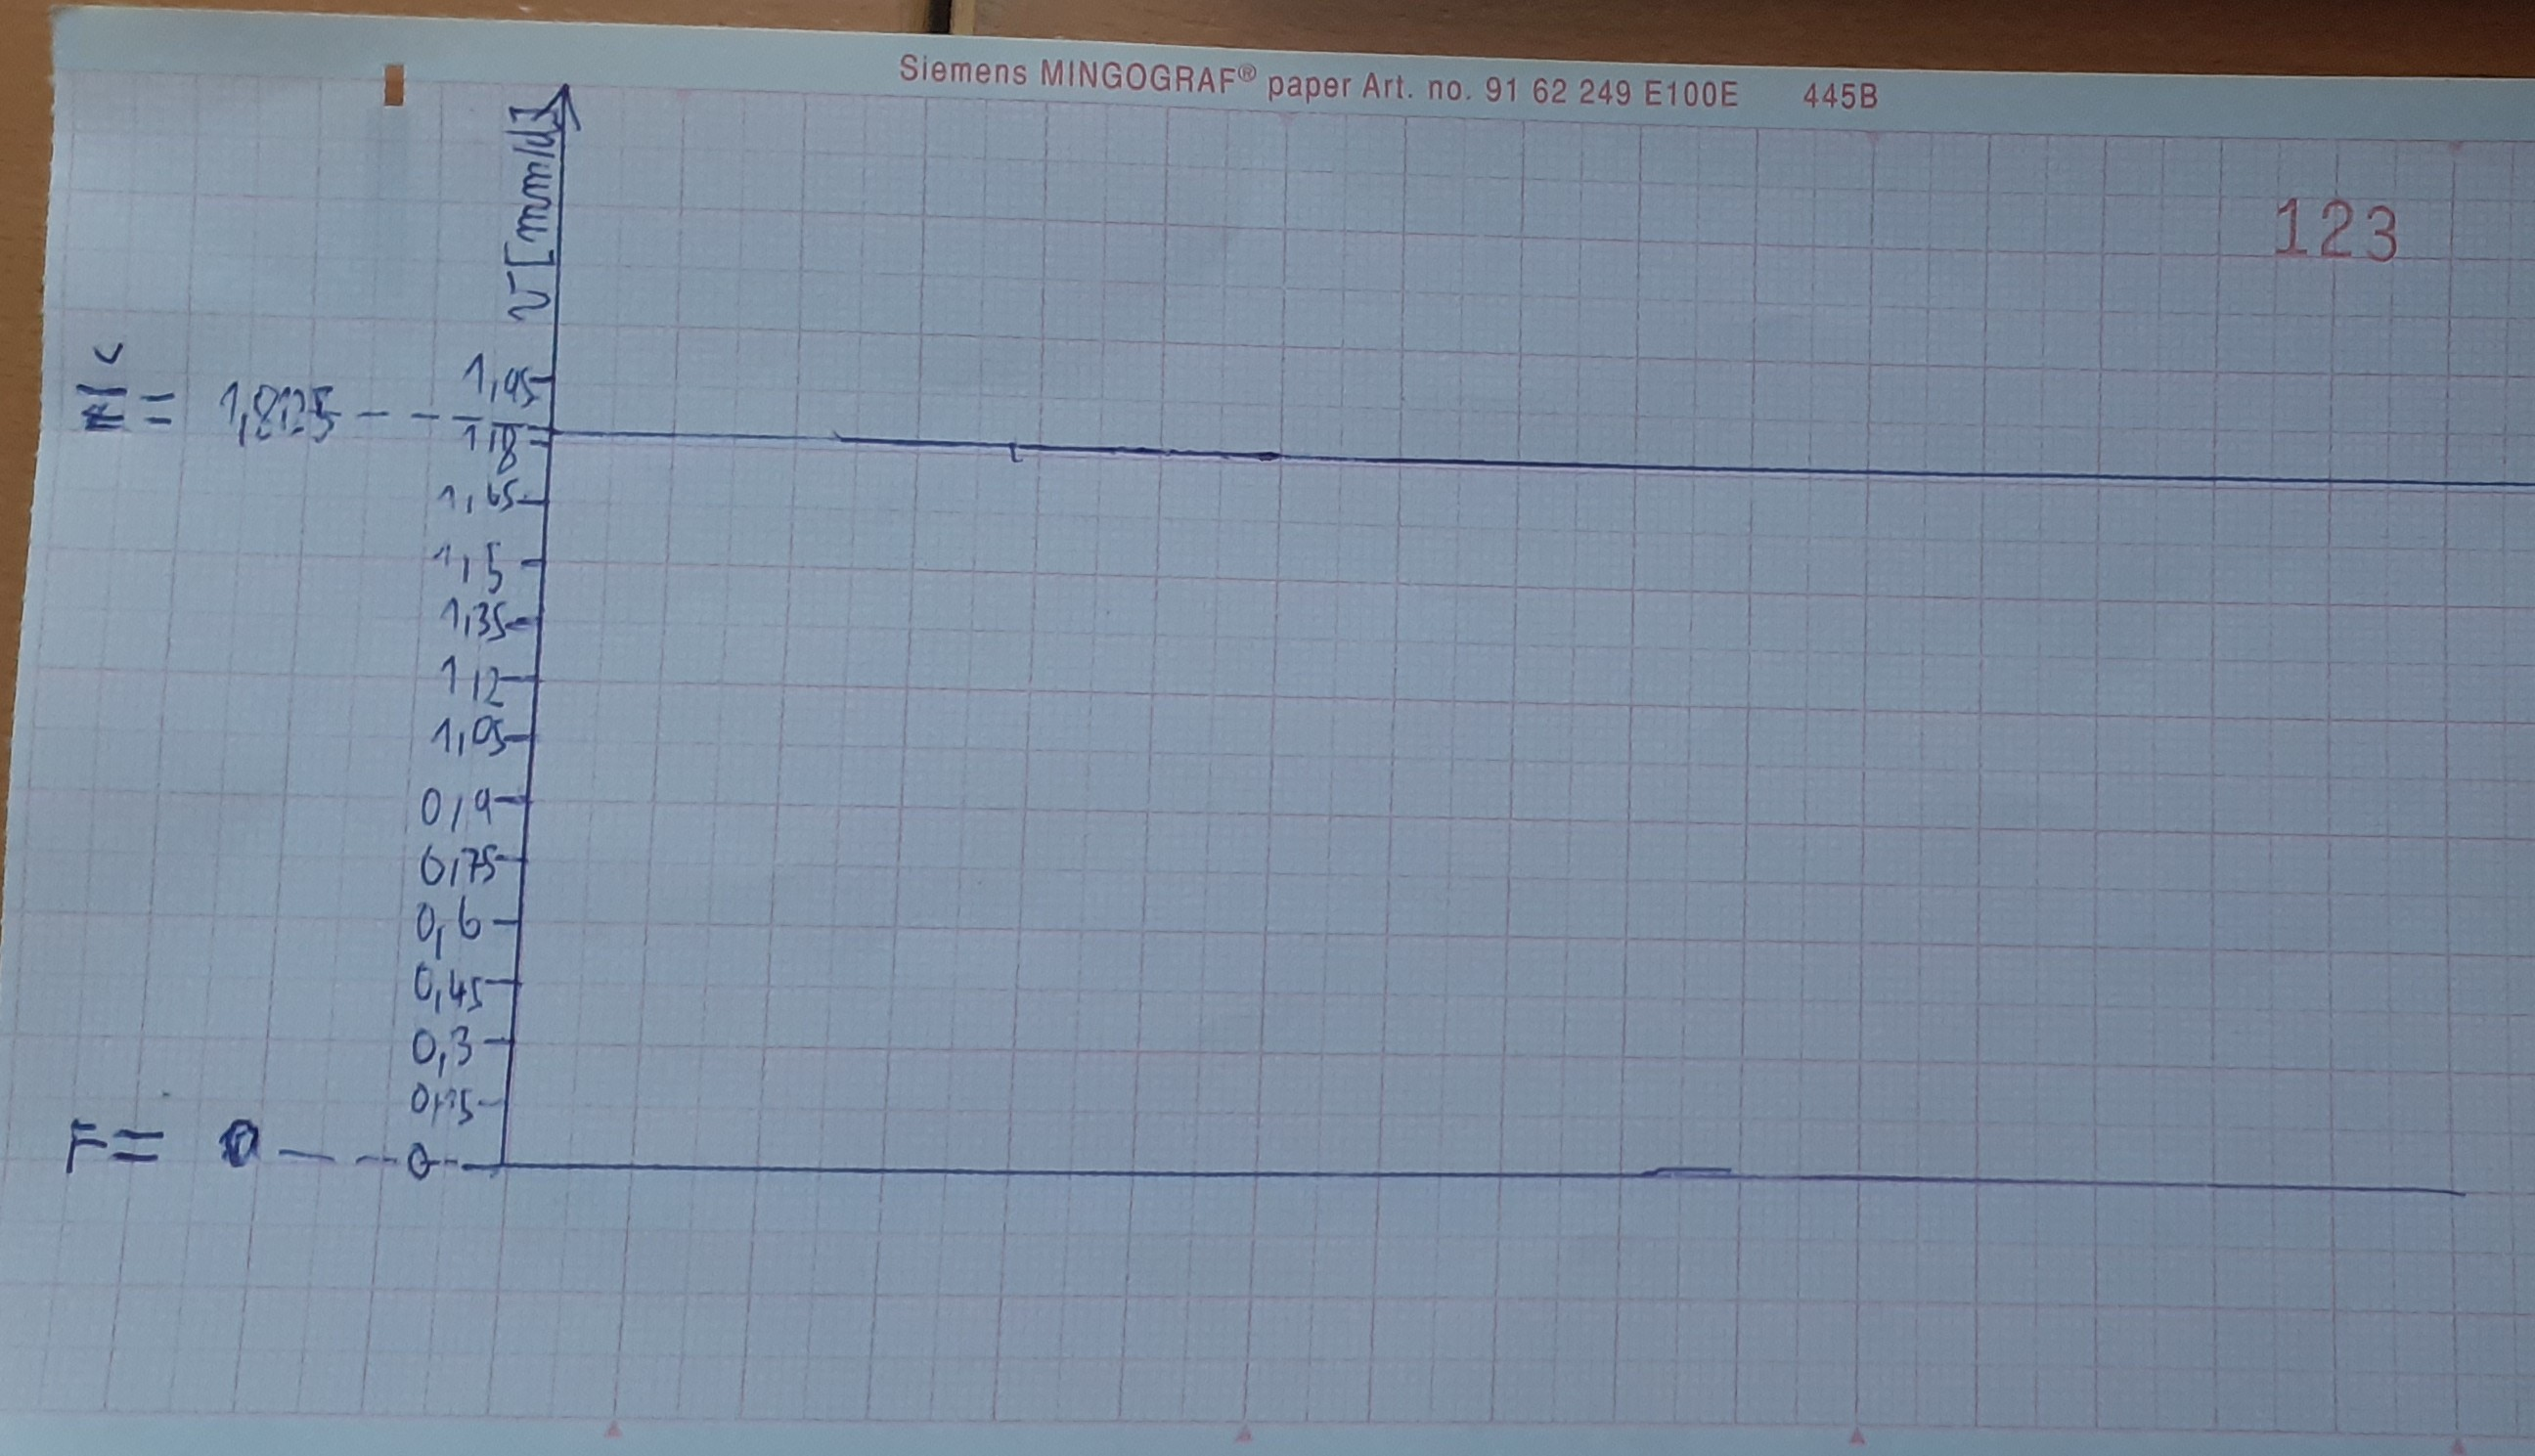
\includegraphics[width=10cm]{graf2.jpeg}
	\caption{Graf $v_z$ a $v_f$ v zásvislosti od ničoho}
\end{figure}

\section{Záver}
Cieľom experimentu bolo zistiť priemernú rýchlosť rastu fazule a žeruchy.
Pri žeruche sme namerali $v_p=1.8125 \frac{mm}{d}$.
Žerucha rástla najrýchlejšie v prvý deň, kedy rástla až rýchlosťou 5 $\frac{mm}{d}$.

Fazuľa nám,žiaľ, však vôbec nevyrástla.
Mohlo to byť spôsobené tým, že bola zahrabaná príliš hlboko, mala príliš veľa/málo vody, semená boli choré alebo nedostatkom svetla.


	
\end{document}
